\documentclass[12pt]{article}
\usepackage{blindtext}
\usepackage{graphicx}
\usepackage{float}
\usepackage[a4paper, total={8in, 10in}]{geometry}
\usepackage{leftindex}
\usepackage{bm}

\title{Report 1}
\author{Ivan Nikolovski}
\date{\today}

\begin{document}
\maketitle
\newpage
\section{T1}
The MDH parameters from task 1 can be seen in the table below
\vspace{1cm}
\begin{table}[htp]
\centering
\large
\begin{tabular}{ |p{2cm}||p{2cm}|p{2cm}|}
 \hline
 i & Link 1 & Link 2\\
 \hline
 $a_i[m]$   & 0   & $l_1$\\
 $d_i[m]$   & 0 & 0\\
 $\alpha_i[rad]$ & 0 & $\delta$\\
 $\theta_i[rad]$ & $q_1$ & $q_2$\\
 \hline
\end{tabular}
\end{table}

\section{T2}
The expressions for the asked matrices can be seen below.
\vspace{1cm}

$\pmb{\leftindex[]^0{T}_1}=\left(\begin{array}{cccc}
\mathrm{cos}\left(q_1 \right) & -\mathrm{sin}\left(q_1 \right) & 0 & 0\\
\mathrm{sin}\left(q_1 \right) & \mathrm{cos}\left(q_1 \right) & 0 & 0\\
0 & 0 & 1 & 0\\
0 & 0 & 0 & 1
\end{array}\right)$

$\pmb{\leftindex[]^1{T}_2}=\left(\begin{array}{cccc}
\mathrm{cos}\left(q_2 \right) & -\mathrm{sin}\left(q_2 \right) & 0 & l_1 \\
\mathrm{sin}\left(q_2 \right) & \mathrm{cos}\left(q_2 \right) & 0 & 0\\
0 & 0 & 1 & \delta \\
0 & 0 & 0 & 1
\end{array}\right)$

$\pmb{\leftindex[]^0{T}_2}=\pmb{\leftindex[]^0{T}_1\leftindex[]^1{T}_2}=\left(\begin{array}{cccc}
\mathrm{cos}\left(q_1 +q_2 \right) & -\mathrm{sin}\left(q_1 +q_2 \right) & 0 & l_1 \,\mathrm{cos}\left(q_1 \right)\\
\mathrm{sin}\left(q_1 +q_2 \right) & \mathrm{cos}\left(q_1 +q_2 \right) & 0 & l_1 \,\mathrm{sin}\left(q_1 \right)\\
0 & 0 & 1 & \delta \\
0 & 0 & 0 & 1
\end{array}\right)$

$\pmb{\leftindex[]^0{T}_{1com}}=\left(\begin{array}{cccc}
\mathrm{cos}\left(q_1 \right) & -\mathrm{sin}\left(q_1 \right) & 0 & {\textrm{lc}}_1 \,\mathrm{cos}\left(q_1 \right)\\
\mathrm{sin}\left(q_1 \right) & \mathrm{cos}\left(q_1 \right) & 0 & {\textrm{lc}}_1 \,\mathrm{sin}\left(q_1 \right)\\
0 & 0 & 1 & 0\\
0 & 0 & 0 & 1
\end{array}\right)$

$\pmb{\leftindex[]^0{T}_{2com}}=\left(\begin{array}{cccc}
\mathrm{cos}\left(q_1 +q_2 \right) & -\mathrm{sin}\left(q_1 +q_2 \right) & 0 & {\textrm{lc}}_2 \,\mathrm{cos}\left(q_1 +q_2 \right)+l_1 \,\mathrm{cos}\left(q_1 \right)\\
\mathrm{sin}\left(q_1 +q_2 \right) & \mathrm{cos}\left(q_1 +q_2 \right) & 0 & {\textrm{lc}}_2 \,\mathrm{sin}\left(q_1 +q_2 \right)+l_1 \,\mathrm{sin}\left(q_1 \right)\\
0 & 0 & 1 & \delta \\
0 & 0 & 0 & 1
\end{array}\right)$

$\pmb{\leftindex[]^0{T}_{EE}}=\left(\begin{array}{cccc}
\mathrm{cos}\left(q_1 +q_2 \right) & -\mathrm{sin}\left(q_1 +q_2 \right) & 0 & l_2 \,\mathrm{cos}\left(q_1 +q_2 \right)+l_1 \,\mathrm{cos}\left(q_1 \right)\\
\mathrm{sin}\left(q_1 +q_2 \right) & \mathrm{cos}\left(q_1 +q_2 \right) & 0 & l_2 \,\mathrm{sin}\left(q_1 +q_2 \right)+l_1 \,\mathrm{sin}\left(q_1 \right)\\
0 & 0 & 1 & \delta \\
0 & 0 & 0 & 1
\end{array}\right)$

$\pmb{\leftindex[]^0{J}_{1,CoM_1}}=\left(\begin{array}{cc}
-{\textrm{lc}}_1 \,\mathrm{sin}\left(q_1 \right) & 0\\
{\textrm{lc}}_1 \,\mathrm{cos}\left(q_1 \right) & 0\\
0 & 0\\
0 & 0\\
0 & 0\\
1 & 0
\end{array}\right)$

$\pmb{\leftindex[]^0{J}_{2,CoM_2}}=\left(\begin{array}{cc}
-{\textrm{lc}}_2 \,\mathrm{sin}\left(q_1 +q_2 \right)-l_1 \,\mathrm{sin}\left(q_1 \right) & -{\textrm{lc}}_2 \,\mathrm{sin}\left(q_1 +q_2 \right)\\
{\textrm{lc}}_2 \,\mathrm{cos}\left(q_1 +q_2 \right)+l_1 \,\mathrm{cos}\left(q_1 \right) & {\textrm{lc}}_2 \,\mathrm{cos}\left(q_1 +q_2 \right)\\
0 & 0\\
0 & 0\\
0 & 0\\
1 & 1
\end{array}\right)$



\section{T3}
The matrices from task 3 can be seen below. The properties from script section 2.4.5 were also both correct in the MATLAB live script.
\\

$\pmb{M(q)}=\left(\begin{array}{cc}
m_2 \,{l_1 }^2 +2\,m_2 \,\mathrm{cos}\left(q_2 \right)\,l_1 \,{\textrm{lc}}_2 +m_1 \,{{\textrm{lc}}_1 }^2 +m_2 \,{{\textrm{lc}}_2 }^2 +\mathrm{I1zz}+\mathrm{I2zz} & m_2 \,{{\textrm{lc}}_2 }^2 +l_1 \,m_2 \,\mathrm{cos}\left(q_2 \right)\,{\textrm{lc}}_2 +\mathrm{I2zz}\\
m_2 \,{{\textrm{lc}}_2 }^2 +l_1 \,m_2 \,\mathrm{cos}\left(q_2 \right)\,{\textrm{lc}}_2 +\mathrm{I2zz} & m_2 \,{{\textrm{lc}}_2 }^2 +\mathrm{I2zz}
\end{array}\right)$


$\pmb{g(q)}=\left(\begin{array}{c}
g\,m_2 \,{\left({\textrm{lc}}_2 \,\mathrm{cos}\left(q_1 +q_2 \right)+l_1 \,\mathrm{cos}\left(q_1 \right)\right)}+g\,{\textrm{lc}}_1 \,m_1 \,\mathrm{cos}\left(q_1 \right)\\
g\,{\textrm{lc}}_2 \,m_2 \,\mathrm{cos}\left(q_1 +q_2 \right)
\end{array}\right)$

$\pmb{C(q,dq)}=\left(\begin{array}{cc}
-{\textrm{dq}}_2 \,l_1 \,{\textrm{lc}}_2 \,m_2 \,\mathrm{sin}\left(q_2 \right) & -{\textrm{dq}}_1 \,l_1 \,{\textrm{lc}}_2 \,m_2 \,\mathrm{sin}\left(q_2 \right)-{\textrm{dq}}_2 \,l_1 \,{\textrm{lc}}_2 \,m_2 \,\mathrm{sin}\left(q_2 \right)\\
{\textrm{dq}}_1 \,l_1 \,{\textrm{lc}}_2 \,m_2 \,\mathrm{sin}\left(q_2 \right) & 0
\end{array}\right)$

\newpage
\section{T4}
Using the following simulink model we can derive the joint angles and velocities which can be seen below in the report.
\begin{figure}[H]
	\centering
	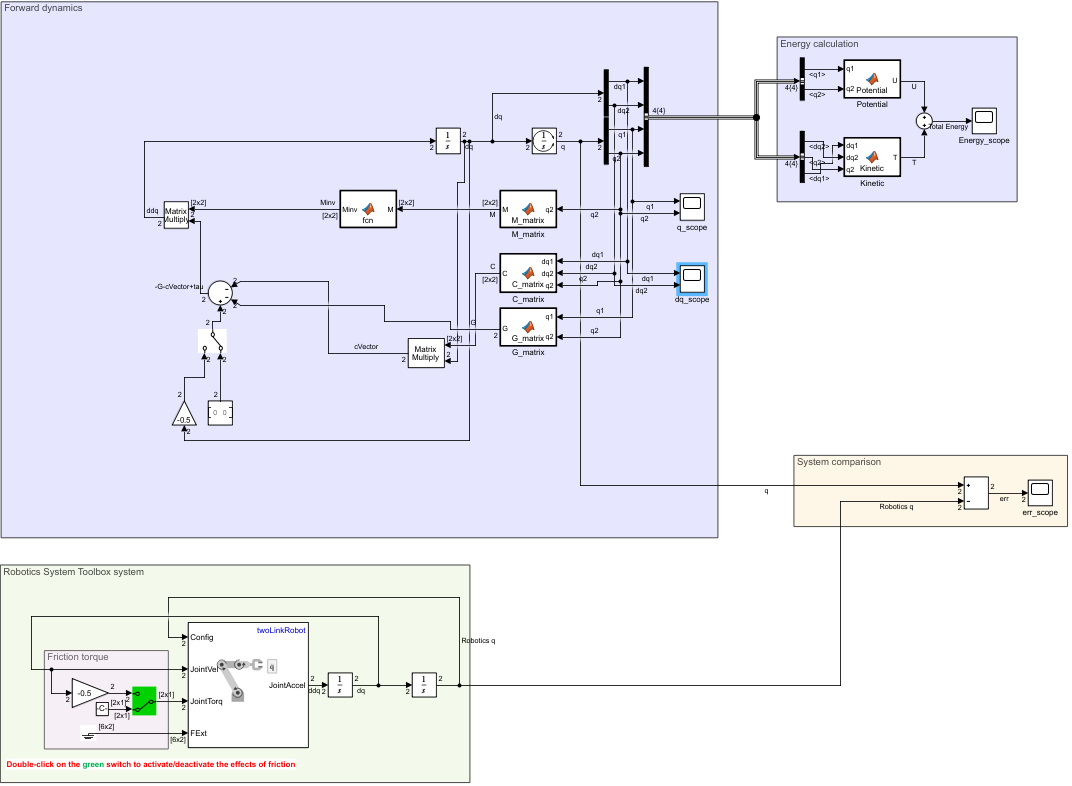
\includegraphics[scale=0.6]{simulinkmodel}
	\caption{Simulink model}
	\label{fig:model}
\end{figure}

\begin{figure}[H]
	\centering
	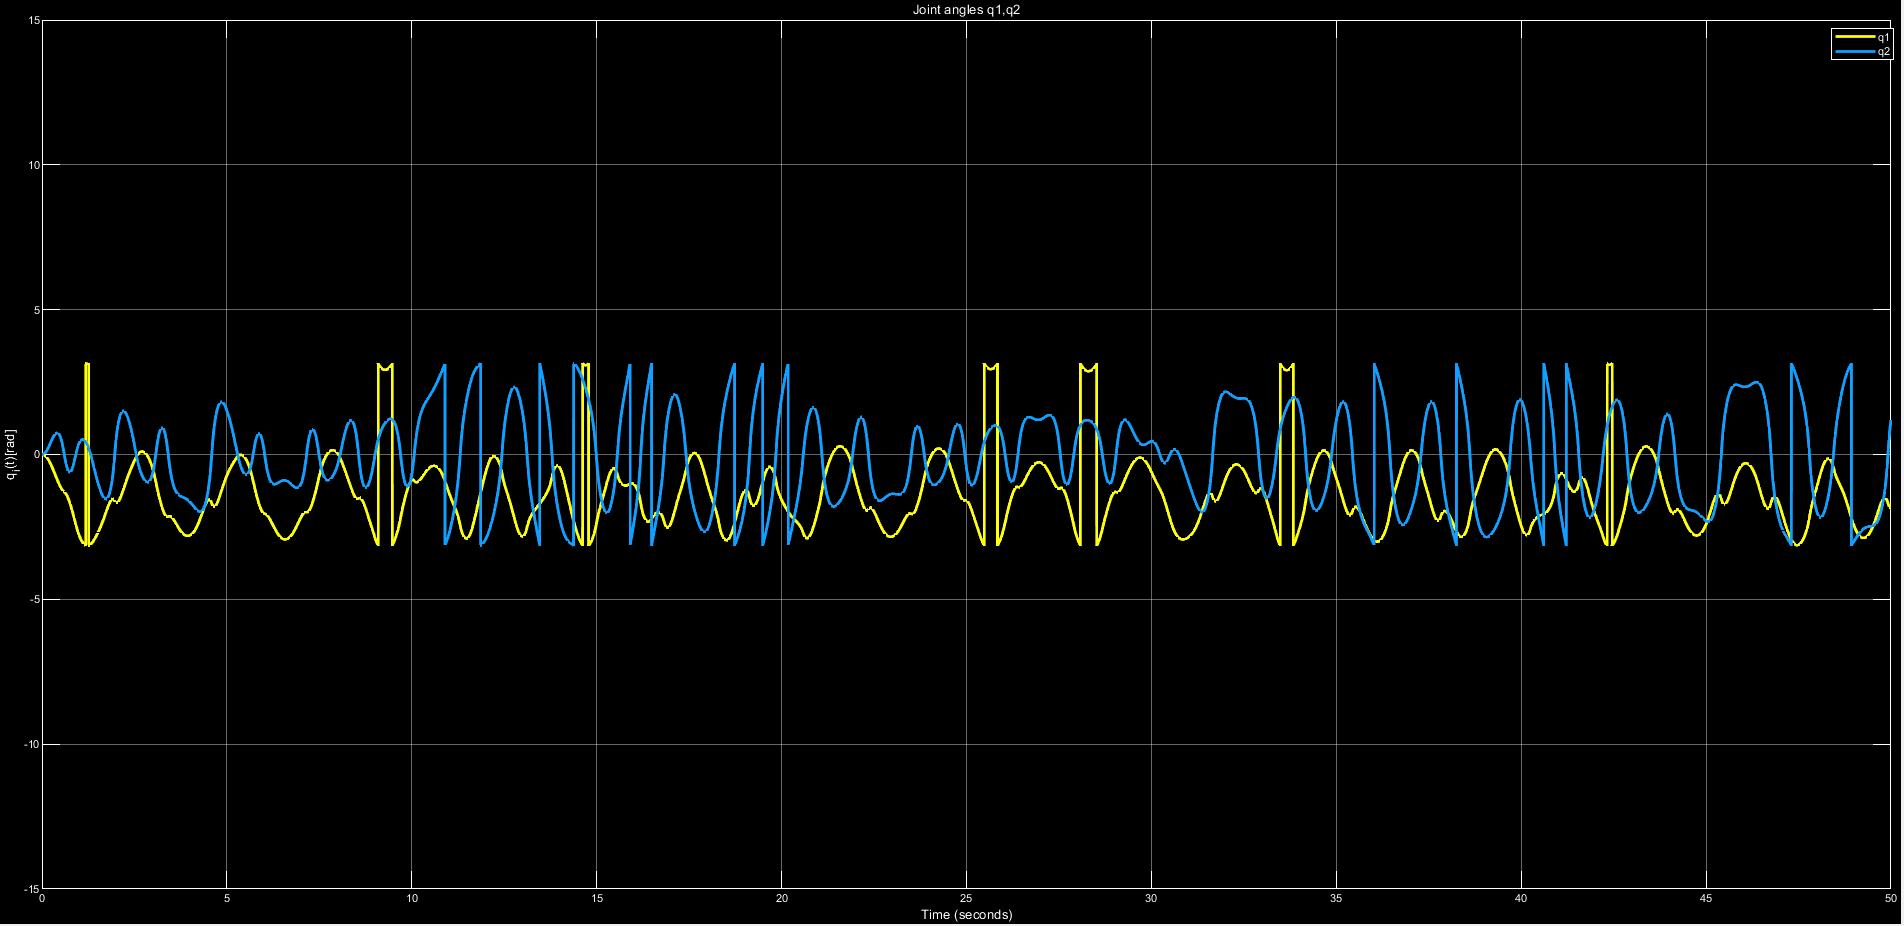
\includegraphics[scale=0.25]{Joint angles}
	\caption{Joint angles over 50 seconds}
\end{figure}

\begin{figure}[H]
	\centering
	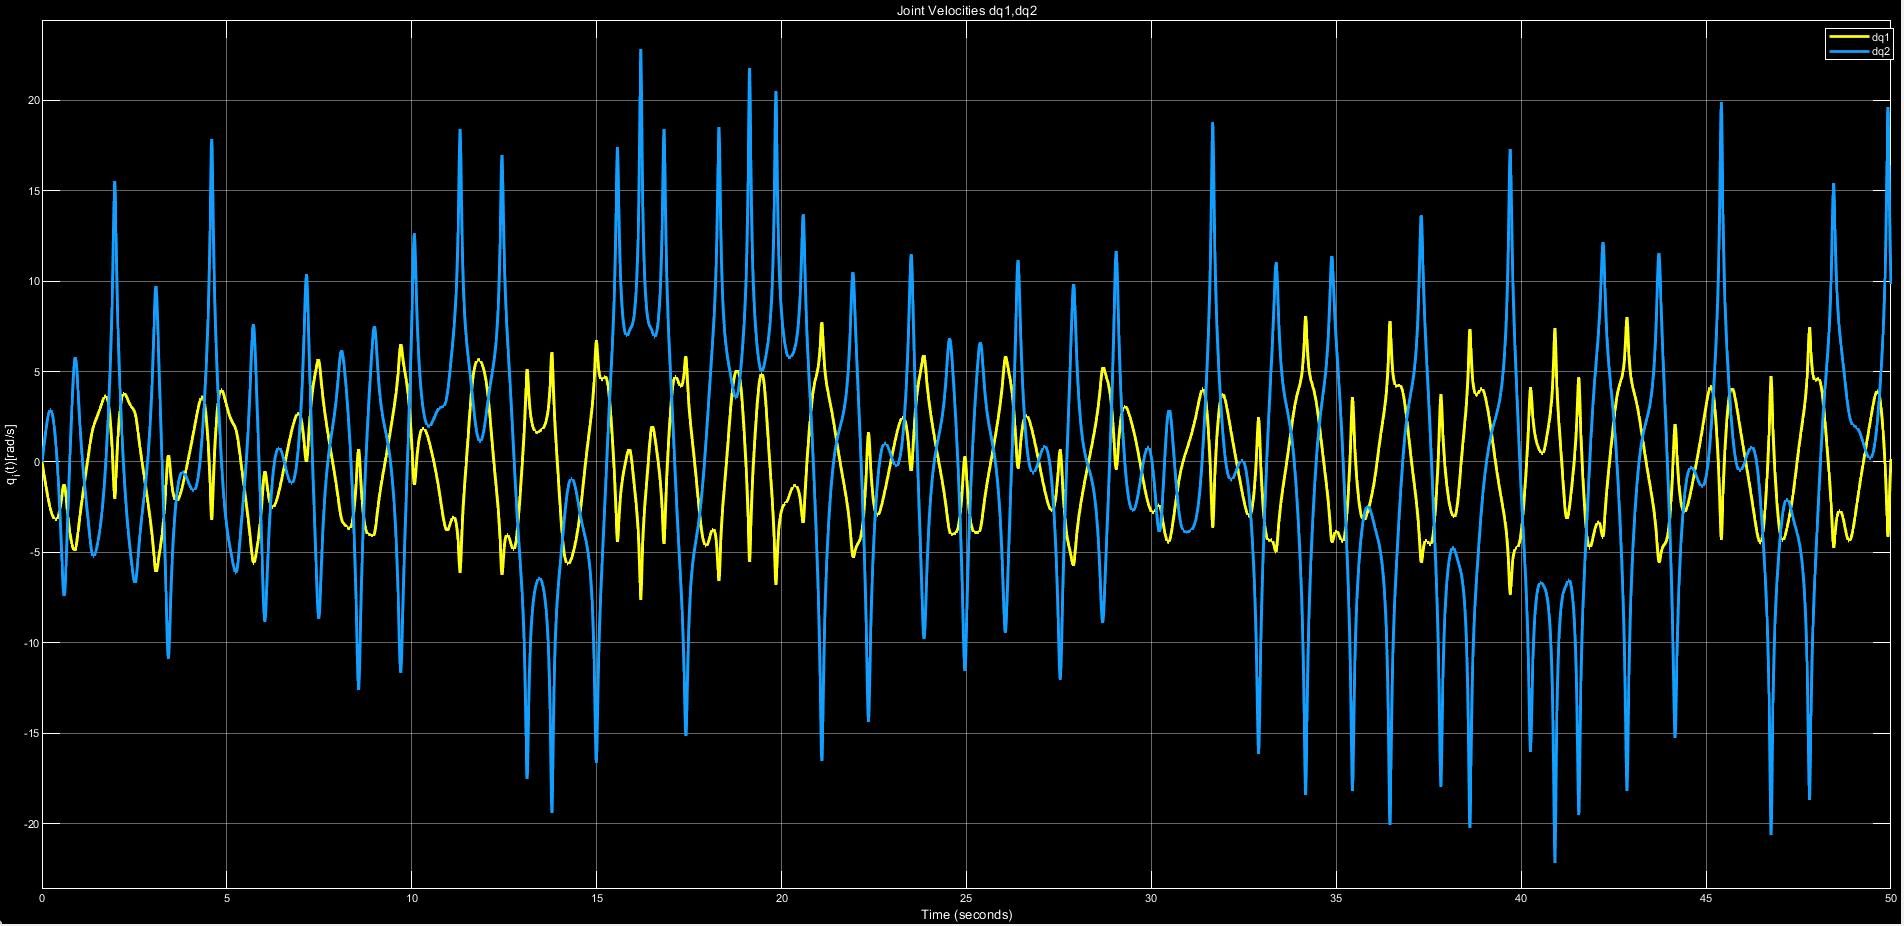
\includegraphics[scale=0.25]{Joint velocities}
	\caption{Joint velocities over 50 seconds}
\end{figure}

\section{T5}
 
The law of conservation of energy states that energy can neither be created nor destroyed - only converted from one form of energy to another. This means that a system always has the same amount of energy, unless it's added from some outside force. In term what this means is that the energy over time should not change unless an external force is added to the system. We can verify this property by looking at the scope for the energy. 

\begin{figure}[H]
	\centering
	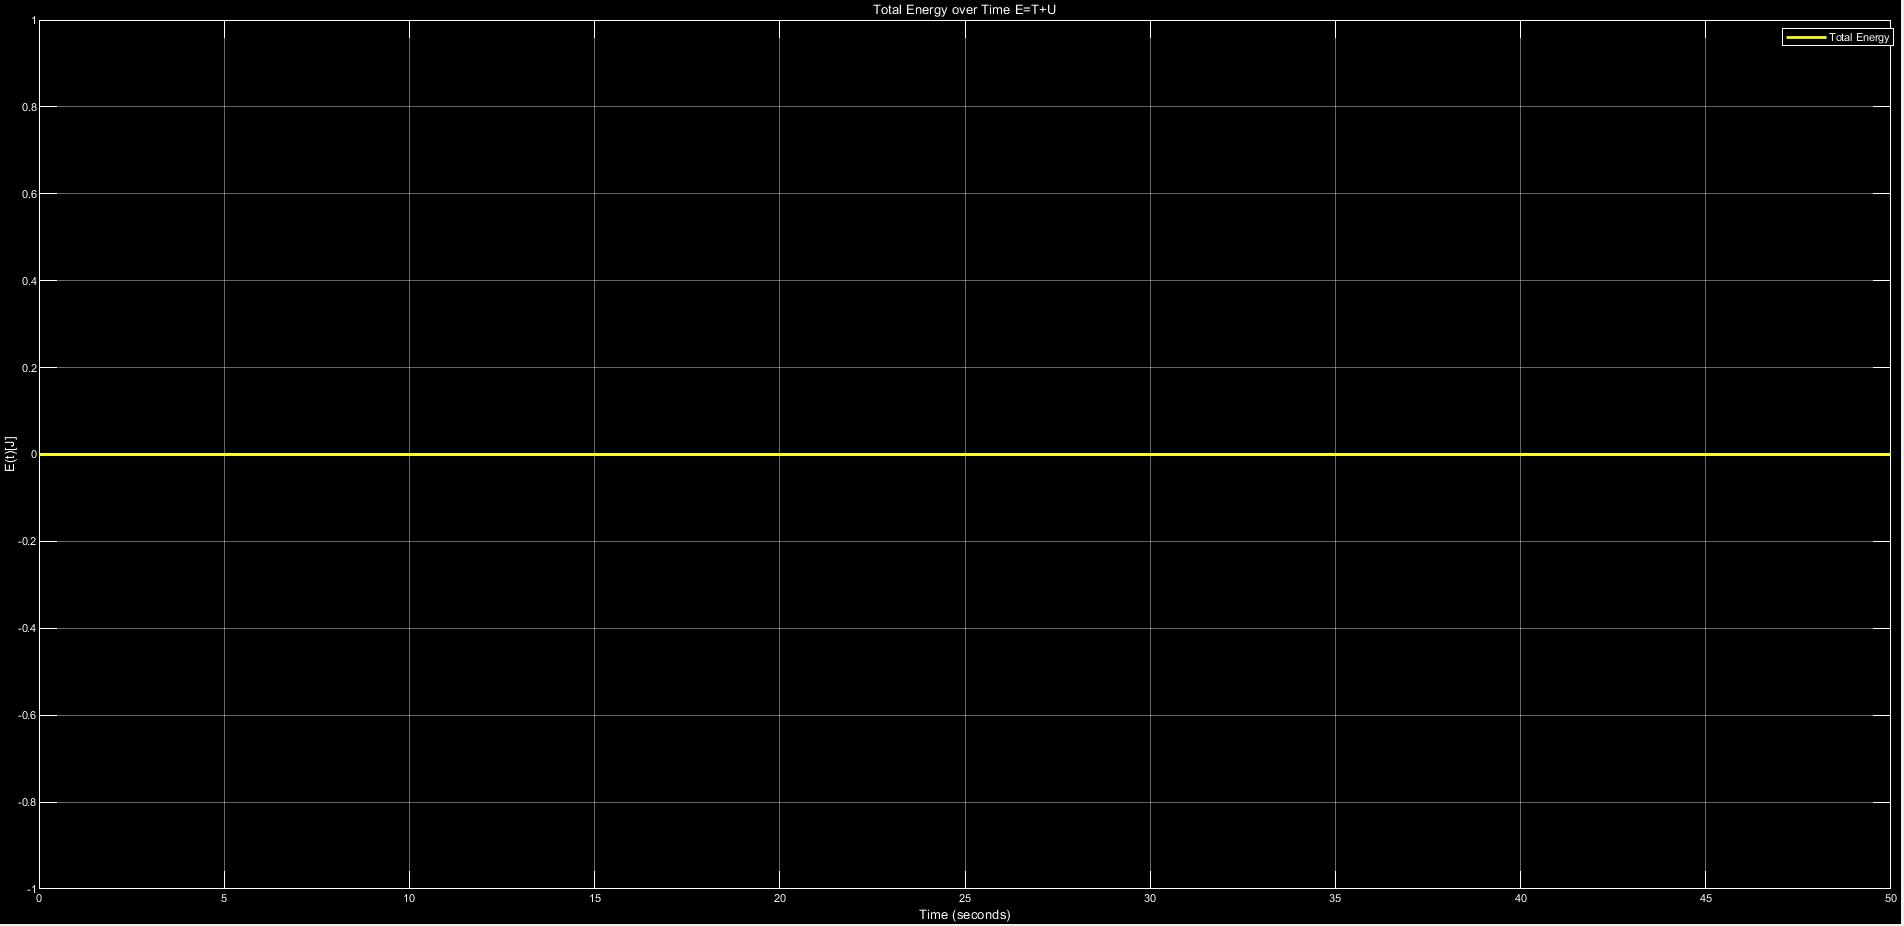
\includegraphics[scale=0.25]{zoomedoutenergyconservation}
	\caption{Energy over time}
\end{figure}

If we were to zoom in we could see that the energy over time is near 0 but not exactly 0 due to MATLABs numerical values. It is somewhere near $0.5*10^{-7}$.

\begin{figure}[H]
	\centering
	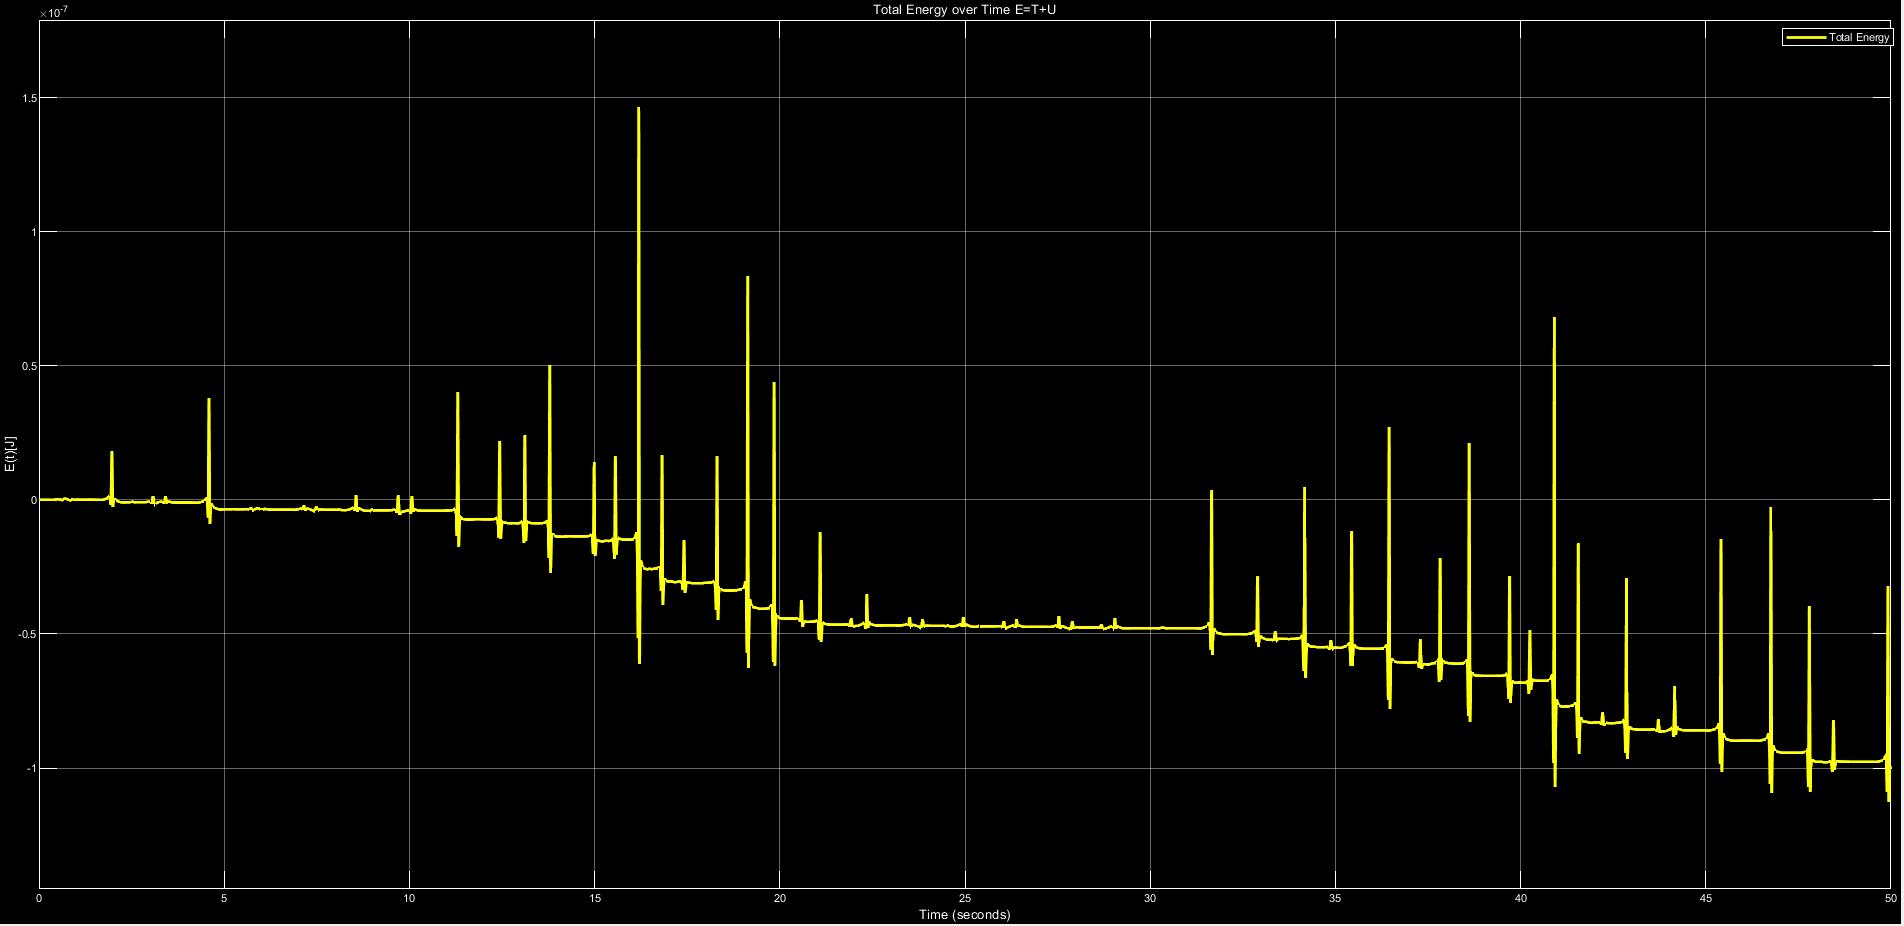
\includegraphics[scale=0.25]{energyconservation}
	\caption{Energy over time zoomed in}
\end{figure}

\newpage


\section{T6}

Here an external force is added to the system-friction. According to the definition above we expect that the energy won't be conserved. And that also happens the energy decreases slightly over time due to the effect of the friction force. This can be seen in the following figure.

\begin{figure}[H]
	\centering
	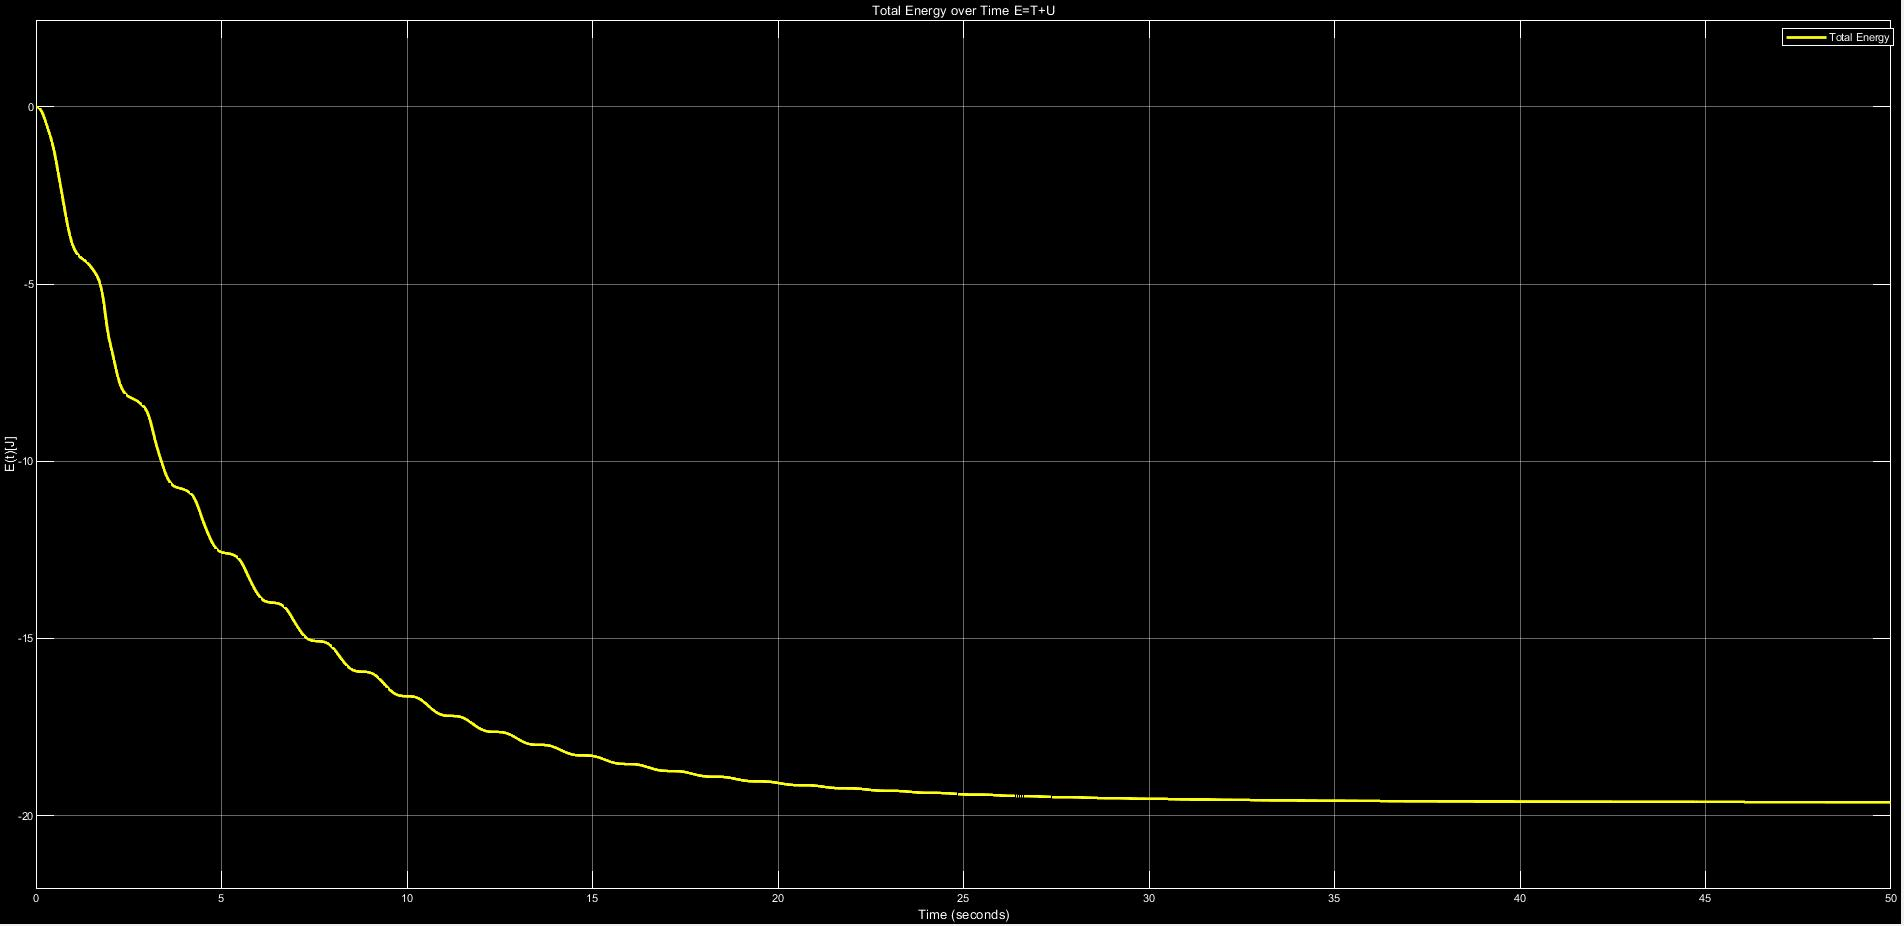
\includegraphics[scale=0.25]{energywithfriction}
	\caption{Energy over time with added friction}
\end{figure}

\end{document}